\section{Teorema de Pick}

\begin{frame}[fragile]{Motivação}

    \begin{itemize}
        \item O Teorema de Pick relaciona a área de uma treliça com o número pontos com
            coordenadas inteiras que estão na borda e o número de pontos com coordenadas 
            inteiras que estão estritamente no interior do polígono
        \pause

        \item Georg Alexander Pick foi o matemático austríaco que descobriu e provou esta
            relação em 1899
        \pause

        \item Se estas quantias forem conhecidas, é possível computar a área do polígono em
            $O(1)$, mesmo sem conhecer seus vértices
        \pause

        \item Conhecidos os vértices, é possível também computar o número de pontos com 
            coordenadas inteiras no interior do polígono em $O(N)$
    \end{itemize}
    
\end{frame}

\begin{frame}[fragile]{Teorema de Pick}

    \metroset{block=fill}
    \begin{block}{Teorema de Pick}
        Seja $P$ uma treliça com área $A$. Seja $I$ e $B$ o número de pontos com coordenadas
            inteiras no interior e na borda de $P$, respectivamente. Então
            \[
                A = I + \frac{B}{2} - 1
            \]
    \end{block}

\end{frame}

\begin{frame}[fragile]{Demonstração do Teorema de Pick}

    \textbf{Demonstração:} Considere que todas as figuras geométricas citadas nesta prova
         tenham vértices com coordenadas inteiras.
        \pause

        A prova do Teorema de Pick é feita em várias etapas:
        \pause
        \begin{enumerate}[(1)]
            \item mostrar que a fórmula é válida para quadrados unitários
        \pause
            \item mostrar que a fórmula vale para qualquer retângulo cujos lados são paralelos
                aos eixos ordenados
        \pause
            \item mostrar que a fórmula vale para triângulos retângulos
        \pause
            \item mostrar que a fórmula vale para triângulos arbitrários
        \pause
            \item mostrar que a fórmula vale para um polígono simples
        \end{enumerate}
\end{frame}

\begin{frame}[fragile]{Demonstração da parte (1)}

    \textbf{(1)} Seja $Q$ um quadrado unitário.

    \begin{figure}
        \centering

        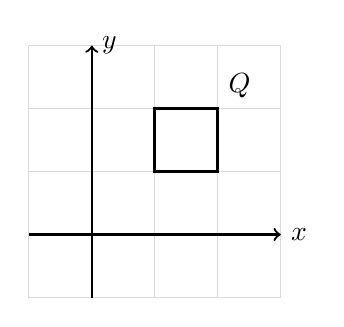
\begin{tikzpicture}
            \begin{scope}[scale=0.8]
            \draw[gray!30] (-1, -1) grid (3,3);

            \draw[thick,->] (-1, 0) -- (3, 0) node[anchor=west] { $x$ };
            \draw[thick,->] (0, -1) -- (0, 3) node[anchor=west] { $y$ };

            \draw[very thick] (1, 1) rectangle (2, 2) node[anchor=south west] { $Q$ };
            \end{scope}
        \end{tikzpicture}
    \end{figure}
        \pause

    Sabemos que $A = 1$. Temos $I = 0$ e $B = 4$, de modo que
    \[
         I + \frac{B}{2} - 1 = 0 + 2 - 1 = 1 = A
    \]
        \pause

    Logo o resultado é válido para quadrados unitários.
\end{frame}

\begin{frame}[fragile]{Demonstração da parte (2)}

    \textbf{(2)} Seja $R$ um retângulo cujos lados são paralelos com os eixos $x$ e $y$ e medem
        $b$ e $h$ unidades, respectivamente.

    \begin{figure}
        \centering

        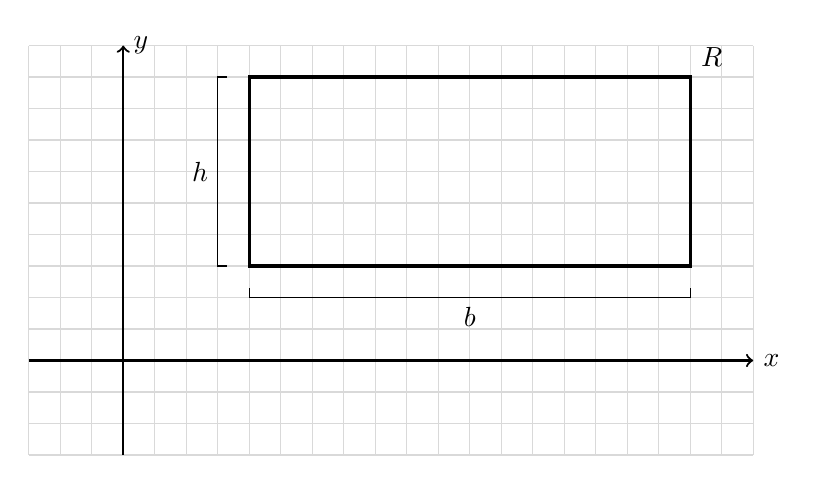
\begin{tikzpicture}
            \begin{scope}[scale=0.4]
            \draw[gray!30] (-3, -3) grid (20,10);

            \draw[thick,->] (-3, 0) -- (20, 0) node[anchor=west] { $x$ };
            \draw[thick,->] (0, -3) -- (0, 10) node[anchor=west] { $y$ };

            \draw[very thick] (4, 3) rectangle (18, 9) node[anchor=south west] { $R$ };

            \draw (3.3, 9) -- (3, 9) -- node[anchor=east] { $ h $ } (3, 3) -- (3.3, 3);
            \draw (4, 2.3) -- (4, 2) -- node[anchor=north] { $ b $ } (18, 2) -- (18, 2.3);
            \end{scope}
        \end{tikzpicture}
    \end{figure}


\end{frame}

\begin{frame}[fragile]{Demonstração da parte (2)}

    Na borda do retângulo há $B = 2(b + 1) + 2(h + 1) - 4$ pontos com coordenadas inteiras, sendo 
    que o termo $-4$ compensa o fato dos vértices estarem sendo contabilizados duas vezes 
    no termo $2(b + 1) + 2(h + 1)$.
        \pause

    No interior do retângulo há $I = (b - 1)(h - 1)$ pontos com coordenadas inteiras.
        \pause

    Sabendo que a área de um retângulo com base $b$ e altura $h$ é $A = bh$, segue que
    \begin{align*}
        I + \frac{B}{2} - 1 &= (b - 1)(h - 1) + \frac{2(b + 1) + 2(h + 1) - 4}{2} - 1 \\
        &= (bh - b - h + 1) - (b + 1 + h + 1 - 2) - 1 \\
        &= bh = A
    \end{align*} \pause
    Portanto o resultado vale para um retângulo cujos lados estão alinhados com os eixos
    ordenados.
\end{frame}

\begin{frame}[fragile]{Demonstração da parte (3)}

    \textbf{(3)} Seja $T$ um triângulo retângulo.

    \begin{figure}
        \centering

        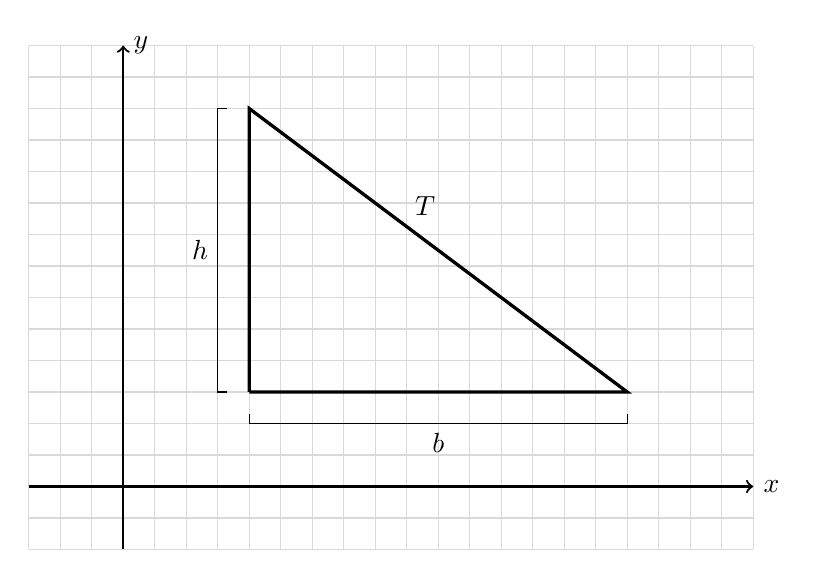
\begin{tikzpicture}
            \begin{scope}[scale=0.4]
            \draw[gray!30] (-3, -2) grid (20,14);

            \draw[thick,->] (-3, 0) -- (20, 0) node[anchor=west] { $x$ };
            \draw[thick,->] (0, -2) -- (0, 14) node[anchor=west] { $y$ };

            \draw[very thick] (4, 3) -- (16, 3) -- node[anchor=south east,yshift=0.3cm,xshift=0.1cm] { $T$ } (4, 12) -- (4, 3);

            \draw (3.3, 12) -- (3, 12) -- node[anchor=east] { $ h $ } (3, 3) -- (3.3, 3);
            \draw (4, 2.3) -- (4, 2) -- node[anchor=north] { $ b $ } (16, 2) -- (16, 2.3);
            \end{scope}
        \end{tikzpicture}
    \end{figure}

\end{frame}


\begin{frame}[fragile]{Demonstração da parte (3)}

    No base do triângulo há $b + 1$ pontos com coordenadas inteiras; já na altura são
    $h + 1$ pontos. 
        \pause

    Seja $d = (b, h)$ o maior divisor comum entre $b$ e $h$. A reta que passa pela hipotenusa
    tem inclinação $m = h'/b'$, onde $b = db', h = dh'$. Isto significa que, para cada unidade
    no sentido $x$ positivo, a altura $y$ varia $m$ unidades.
        \pause

    Assim, a equação da reta é dada por $y = m(x - x_0) + y_0$, onde $x_0$ e $y_0$ tem coordenadas 
    inteiras. Assim, os valores de $x$ serão inteiros quando $(x - x_0)$ assumir valores múltiplos 
    de $b'$.
        \pause
        
    A hipotenusa começa com $y = y_0$ e termina com $y = y_1$ inteiro, com $y_1 - y_0 = h$.
    Em $y_0$ temos $x = x_0$, ou seja, $(x - x_0) = 0 = 0\cdot b'$. Em $y_1$ temos
    \begin{align*}
       y_1 = y_0 + h = m(x - x_0) + y_0 = \frac{h'}{b'}(x - x_0) + y_0
    \end{align*}
             
\end{frame}

\begin{frame}[fragile]{Demonstração da parte (3)}

    Assim,

    \begin{align*}
        \frac{h'}{b'}(x - x_0) &= h\\
        (x - x_0) &= h\frac{b'}{h'} = b'\cdot d,
    \end{align*}

    de modo que o valor de $y$ será inteiro em $d + 1$ múltiplos de $b'$, a saber: $0, 1, \ldots, d$.
        \pause

    Levando em consideração que os vértices são contados duas vezes cada, o número de pontos $B$
    com coordenadas inteiras na borda de $T$ é igual a
    \[
        B = (b + 1) + (h + 1) + (d + 1) - 3 = b + h + d
    \] \pause
    O número de pontos com coordenadas inteiras $I$ no interior de $T$ é igual a metade do
    número de pontos no interior do retângulo com base $b$ e altura $h$, exceto os pontos sobre
    a diagonal e que são interiores, isto é, $(d + 1) - 2 = d - 1$.
\end{frame}

\begin{frame}[fragile]{Demonstração da parte (3)}
    Logo,
    \[
        I = \frac{(b - 1)(h - 1) - (d - 1)}{2} = \frac{bd - b - h - d + 2}{2}
    \]
        \pause

    Sabendo que a área de um triângulo retângulo com base $b$ e altura $h$ é dada por
    $A = bh/2$, segue que
    \begin{align*}
        I + \frac{B}{2} - 1 &= \frac{bd - b - h - d + 2}{2} + \frac{b + d + h}{2} - 1 \\
        &= \frac{bh}{2} + \frac{2}{2} - 1 = \frac{bh}{2} = A,
    \end{align*}

    portanto o resultado vale para $T$.
\end{frame}

\begin{frame}[fragile]{Demonstração da parte (4)}

    \textbf{(4)} Seja $T$ um triângulo qualquer.

    \begin{figure}
        \centering

        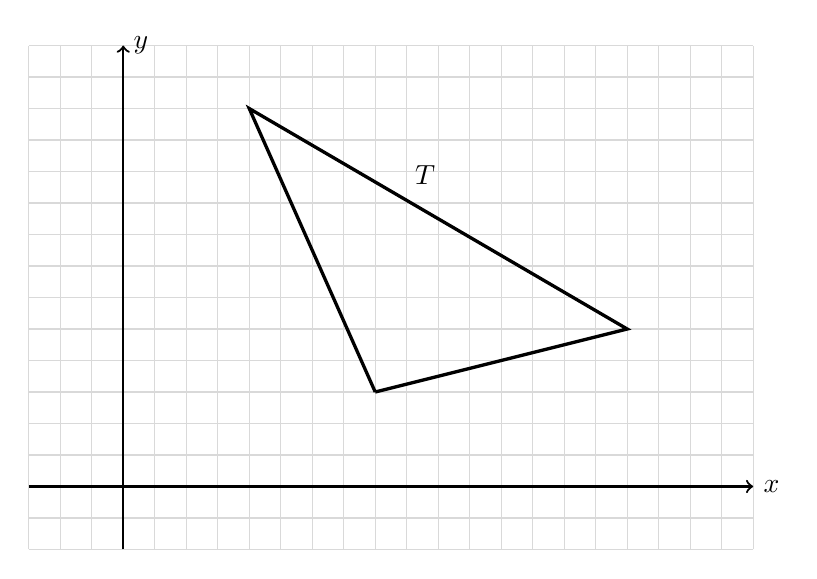
\begin{tikzpicture}
            \begin{scope}[scale=0.4]
            \draw[gray!30] (-3, -2) grid (20,14);

            \draw[thick,->] (-3, 0) -- (20, 0) node[anchor=west] { $x$ };
            \draw[thick,->] (0, -2) -- (0, 14) node[anchor=west] { $y$ };

            \draw[very thick] (8, 3) -- (16, 5) -- node[anchor=south east,yshift=0.3cm,xshift=0.1cm] { $T$ } (4, 12) -- (8, 3);

            %\draw (3.3, 12) -- (3, 12) -- node[anchor=east] { $ h $ } (3, 3) -- (3.3, 3);
            %\draw (4, 2.3) -- (4, 2) -- node[anchor=north] { $ b $ } (16, 2) -- (16, 2.3);
            \end{scope}
        \end{tikzpicture}
    \end{figure}

\end{frame}

\begin{frame}[fragile]{Demonstração da parte (4)}

    Seja $x_{min}, y_{min}, x_{max}, y_{max}$ os valores mínimos e máximos das coordenadas dos
        vértices. É possível construir um retângulo com base $b = x_{max} - x_{min}$ e
        altura $h = y_{max} - y_{min}$ através da união de $T$ com três triângulos retângulos
        $T_1, T_2$ e $T_3$
        \pause

    \begin{figure}
        \centering

        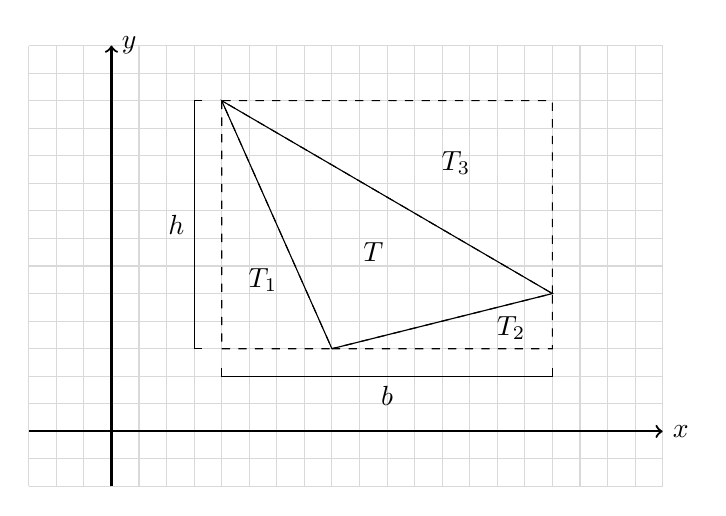
\begin{tikzpicture}
            \begin{scope}[scale=0.35]
            \draw[gray!30] (-3, -2) grid (20,14);

            \draw[thick,->] (-3, 0) -- (20, 0) node[anchor=west] { $x$ };
            \draw[thick,->] (0, -2) -- (0, 14) node[anchor=west] { $y$ };

            \draw[dashed] (4, 3) -- (8, 3) -- (4, 12) -- (4, 3);
            \node at (5.5, 5.5) { $T_1$ };

            \draw[dashed] (8, 3) -- (16, 3) -- (16, 5) -- (8, 3);
            \node at (14.5, 3.75) { $T_2$ };

            \draw[dashed] (16, 5) -- (16, 12) -- (4, 12) -- (16, 5);
            \node at (12.5, 9.75) { $T_3$ };

            \draw (8, 3) -- (16, 5) -- (4, 12) -- (8, 3);
            \node at (9.5, 6.5) { $T$ };

            \draw (3.3, 12) -- (3, 12) -- node[anchor=east] { $ h $ } (3, 3) -- (3.3, 3);
            \draw (4, 2.3) -- (4, 2) -- node[anchor=north] { $ b $ } (16, 2) -- (16, 2.3);
            \end{scope}
        \end{tikzpicture}
    \end{figure}

\end{frame}

\begin{frame}[fragile]{Demonstração da parte (4)}

    O número de pontos com coordenadas inteiras no interior do retângulo $R$ é igual a
    \[
        I_R = I_{T_1} + I_{T_2} + I_{T_3} + I_{T} + (B_{T} - 3),
    \]
    onde $B_T$ é o número de pontos com coordenadas inteiras na borda de $T$
        \pause

    Por outro lado,
    \[
        B_R = B_{T_1} + B_{T_2} + B_{T_3} - B_{T}
    \]
        \pause

    Como o resultado vale para retângulos e triângulos retângulos, e observando que
    \[
        A_T = A_R - (A_{T_1} + A_{T_2} + A_{T_3}),
    \]

\end{frame}

\begin{frame}[fragile]{Demonstração da parte (4)}

    segue que
    \begin{align*}
        A_T &= \left( I_R - \frac{B_R}{2} - 1\right) - \left[
        \left( I_{T_1} + I_{T_2} + I_{T_3} \right) +
        \left( \frac{B_{T_1} + B_{T_2} + B_{T_3}}{2}\right) - 3\right] \\
        &= \left(I_R - I_{T_1} + I_{T_2} + I_{T_3} \right) +
        \left( \frac{B_R - B_{T_1} - B_{T_2} - B_{T_3}}{2}\right) + 2\\
        &= \left(I_T + B_T - 3 \right) -
        \left( \frac{B_T}{2}\right) + 2\\
        &= I_T + \frac{B_T}{2} - 1,
    \end{align*}
    logo o teorema é verdadeiro para um triângulo $T$ qualquer.

\end{frame}

\begin{frame}[fragile]{Demonstração da parte (5)}

    \textbf{(5)} A última parte é demonstrada por indução. 
    \pause

    Seja $P$ um polígono simples. O caso base ocorre para um triângulo, e o resultado é 
    verdadeiro para qualquer triângulo $T$, conforme já demonstrado.
    \pause

    Suponha que o resultado seja verdadeiro para qualquer polígono simples como $m\geq 3$ lados.
    Seja $P$ um polígono simples com $m + 1$ lados. Como $P$ é simples, ele pode ser 
        decomposto na forma $P = T\cup Q$, onde $T$ é um triângulo e $Q$ um polígono simples
        com $m$ lados, ambos compartilhando uma aresta em comum. Considere que o número de
        pontos com coordenadas inteiras na aresta comum de $T$ e $Q$, internos em $P$, seja igual a $k$.
    \pause

    Desde modo, $I_P = I_T + I_Q + k$ e $B_P = B_T + B_Q - 2k - 2$. Veja a figura a seguir.

\end{frame}

\begin{frame}[fragile]{Demonstração da parte (5)}

    \begin{figure}
        \centering

        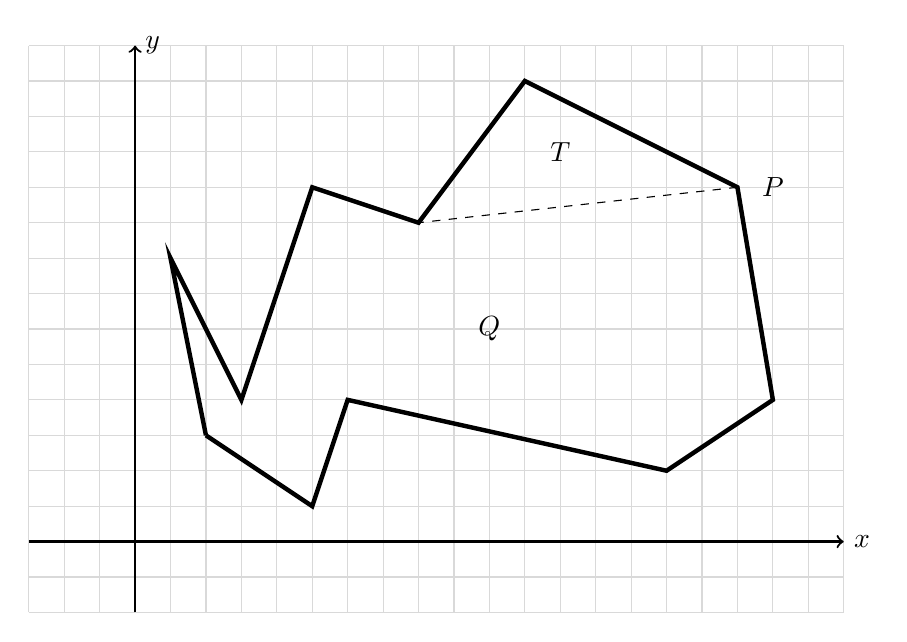
\begin{tikzpicture}
            \begin{scope}[scale=0.45]
            \draw[gray!30] (-3, -2) grid (20,14);

            \draw[thick,->] (-3, 0) -- (20, 0) node[anchor=west] { $x$ };
            \draw[thick,->] (0, -2) -- (0, 14) node[anchor=west] { $y$ };

            \draw[ultra thick] (2, 3) -- (5, 1) -- (6, 4) -- (15, 2) -- (18, 4)
                -- (17, 10) -- (11, 13) -- (8, 9) -- (5, 10) -- (3, 4) -- (1, 8) -- (2, 3);

            \draw[dashed] (17, 10) -- (8, 9);

            \node at (18, 10) { $P$ };
            \node at (12, 11) { $T$ };

            \node at (10, 6) { $Q$ };

            \end{scope}
        \end{tikzpicture}
    \end{figure}

\end{frame}
\begin{frame}[fragile]{Demonstração da parte (5)}
    Assim,
    \begin{align*}
        A_P &= A_T + A_Q \\
            & = \left(I_T + \frac{B_T}{2} - 1\right) 
            + \left(I_Q + \frac{B_Q}{2} - 1\right) \\
            &= \left(I_T + I_Q + k\right) + 
            \left(\frac{B_T + B_Q}{2} - k - 1 \right) - 1\\
            &= I_P + \left(\frac{B_T + B_Q - 2k - 2}{2} \right) - 1\\
            &= I_P + \left(\frac{B_P}{2} \right) - 1,
    \end{align*}
    \pause

    Portanto o resultado é válido para qualquer polígono simples.

\begin{flushright}
$\square$
\end{flushright}

\end{frame}
